\clearpage
\renewcommand{\appendixname}{Supplementary Materials} 
\appendix


\begin{figure*}[tb!]
    \centering
    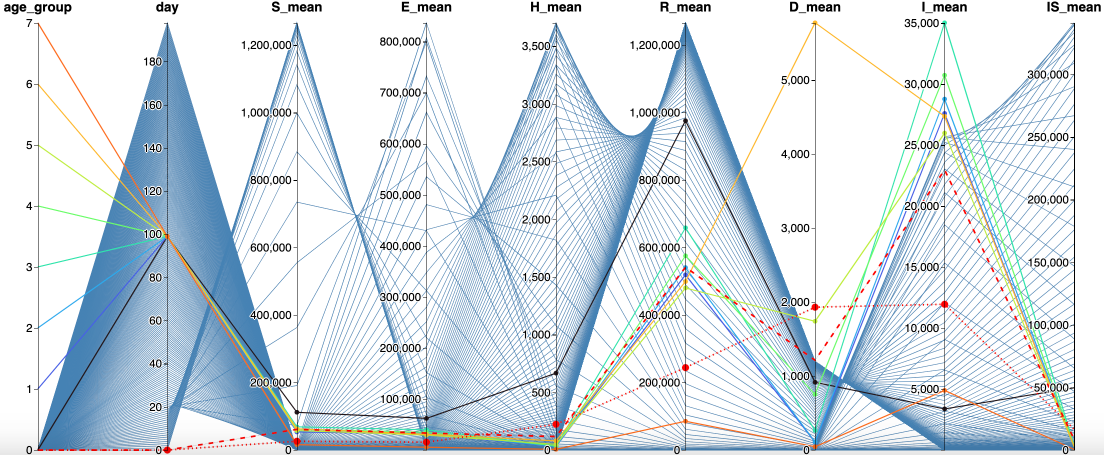
\includegraphics[width=\linewidth]{pc2.png}
    \caption{A parallel coordinates plot depicting the model outcomes by age group. As requested by the modelers, the mean value of 160 predictions generated by each input configuration, as well as for each age group, was computed and rendered here. Each axis represents one variable from the outcome and \textcolor{SteelBlue4}{its value}.
    Each age group is mapped to a color, the dashed red line {\textcolor{red}{
    \rule[0.3ex]{0.2cm}{0.5pt}\hspace{0.1cm}
    \rule[0.3ex]{0.2cm}{0.5pt}\hspace{0.1cm}
    \rule[0.3ex]{0.2cm}{0.5pt}\hspace{0.1cm}
    }}
    represents the average value, and the dotted red line \textcolor{red}{\textcolor{red}{
    \rule[0.3ex]{0.05cm}{0.1pt}\hspace{0.05cm}
    \rule[0.3ex]{0.05cm}{0.1pt}\hspace{0.05cm}
    \rule[0.3ex]{0.05cm}{0.1pt}\hspace{0.05cm}
    }} represents the standard deviation.
    }

\end{figure*}